%%%%%%%%%%%%%%%%%%%%%%%%%%%%%%%%%%%%%%%%%%%%%%%%%%%%%%%%%%%%%%%%%
%_____________ ___    _____  __      __ 
%\____    /   |   \  /  _  \/  \    /  \  Institute of Applied
%  /     /    ~    \/  /_\  \   \/\/   /  Psychology
% /     /\    Y    /    |    \        /   Zuercher Hochschule 
%/_______ \___|_  /\____|__  /\__/\  /    fuer Angewandte Wissen.
%        \/     \/         \/      \/                           
%%%%%%%%%%%%%%%%%%%%%%%%%%%%%%%%%%%%%%%%%%%%%%%%%%%%%%%%%%%%%%%%%
%
% Project     : Seminararbeit
% Title       : 
% File        : einfluss.tex Rev. 00
% Date        : 10.10.2012
% Author      : Till J. Ernst
%
%%%%%%%%%%%%%%%%%%%%%%%%%%%%%%%%%%%%%%%%%%%%%%%%%%%%%%%%%%%%%%%%%
\thispagestyle{empty}
\chapter{Einfluss Sozialer Medien auf das Subjektive Wohlbefinden}\label{chap.einfluss}
Text blablabla...
%Abbildung von ConceptMap SWB und SM
\begin{figure}[H]
	\centering
		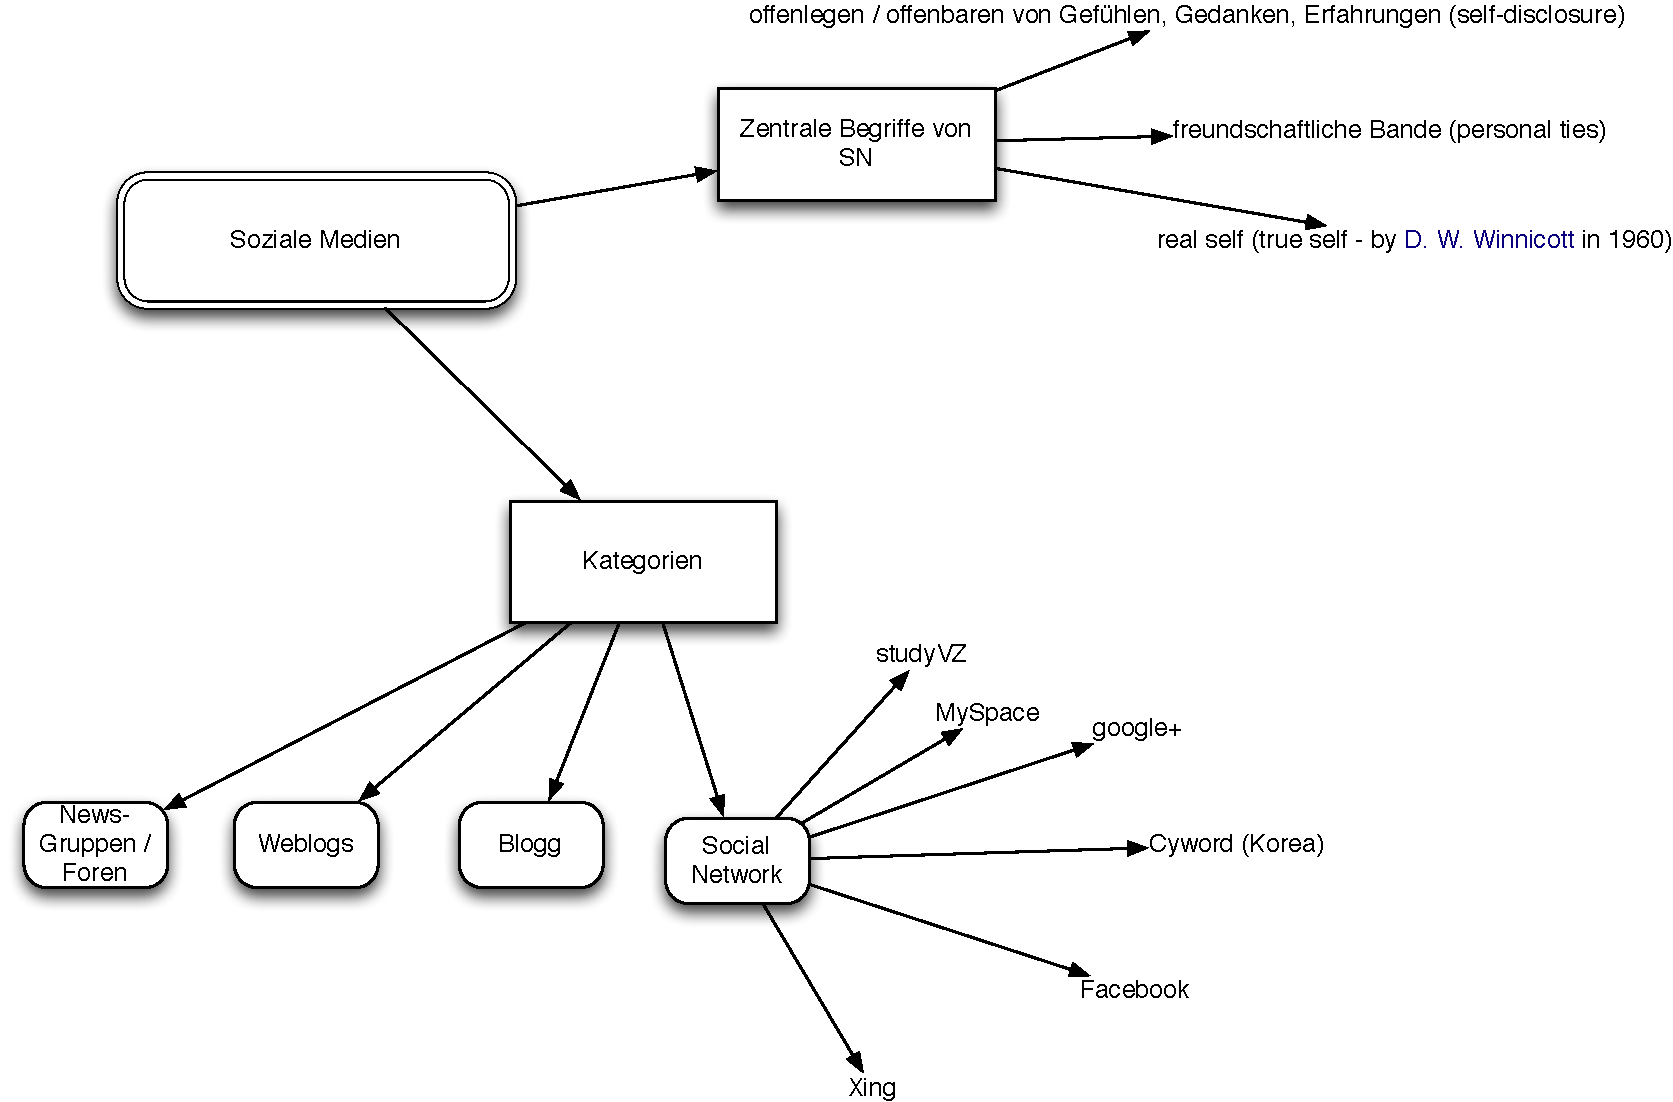
\includegraphics[width=0.8\textwidth]{images/grafiken/02_SozialeNetzwerke_Ueberblick.pdf}
	\caption{ConceptMap - Subjektives Wohlbefinden und Social Media}
	\label{fig.ConceptMapSwbSm}
\end{figure}

